
In a typical imaging system, before arriving at the sensor, the incident light is collected and focused through an optical system first. Lenses, most common optical components, have a resolving power of their own, which has to match the resolution of the sensor and is fundamentally limited by the nature of light. 

Upon encountering an opening (\textit{aperture}), the incident light diffracts into a series of concentric waves propagated concentrically around the corners. Assuming a perfectly circular aperture, wavefronts belonging to one point in object space will produce a diffraction pattern with a bright spot in the middle, surrounded by concentrical rings of reduced intensities. The diameter of such pattern, \textit{Airy disk}, is given through:

\begin{displaymath}
    D_{Airy} \approx 2.44 \frac{\lambda {f}'}{D} = 2.44 \lambda  k
\end{displaymath}

with $\lambda$ being the wavelength of the incoming light, ${f}'$ the focal length, and $D$ the diameter of the entrance pupil, respectively; in lenses, which can be treated as a circular aperture of respective diameter, the \textit{focal ratio} serves as the \textit{nominal aperture} $k$, or \textit{f-stop}. 

\begin{figure}[h]
  \centering
  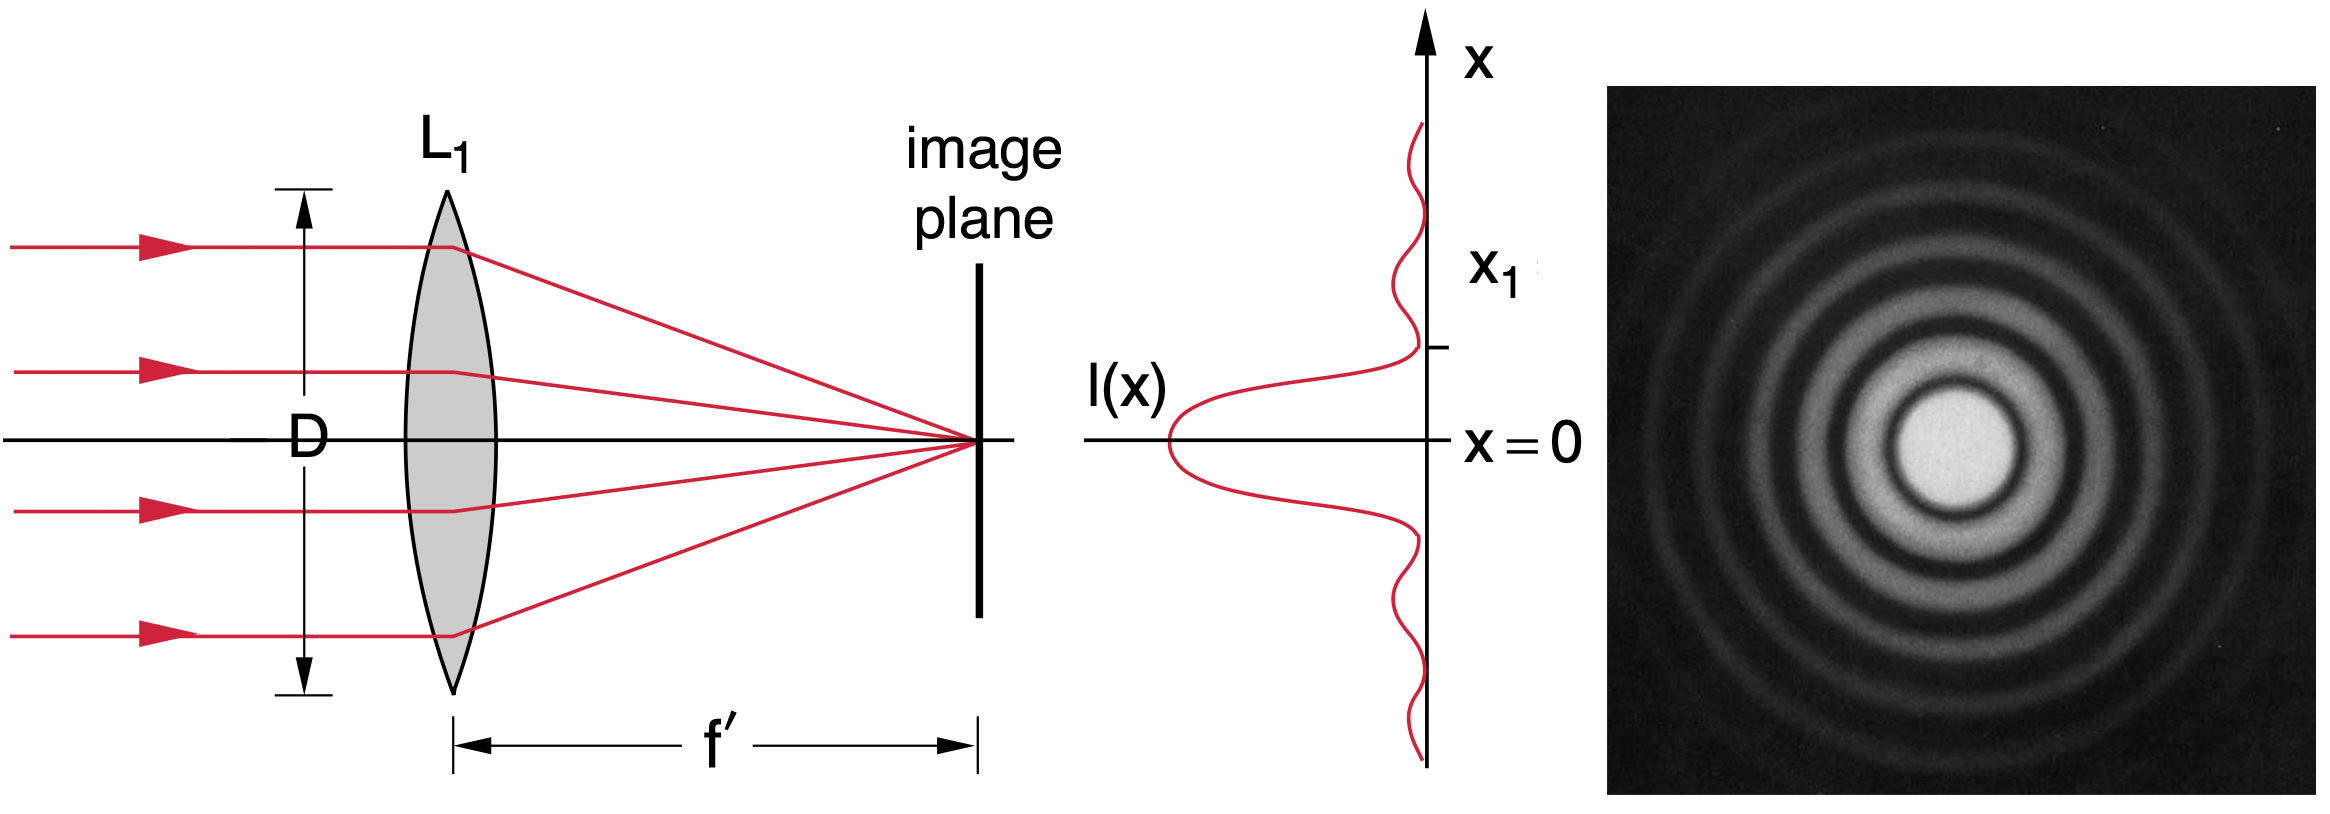
\includegraphics[width=\linewidth]{imgs/optics/airy.png}
  \caption{Airy disk pattern caused through lens diffraction of a point source, via \cite{Cagnet1962}, and and the corresponding distribution of intensities, \cite{Demtroeder2018}.}
  \label{fig:airy}
  \Description{The bundle of light passing through a lens, acting as an aperture. Through diffraction, the points in the object plane are depicted as a concentric wave-like pattern of diminishing intensities.}
\end{figure}

For two distant neighboring points, the half-angle ${\delta}'_{min}$ subtended by the numerical aperture (represented by the lens) is too small. Thus, the two objects will not be perceived as separate entities; as their intensity functions coincide at their respective minimums, the disks will start to overlap. 

\begin{figure}[h]
  \centering
  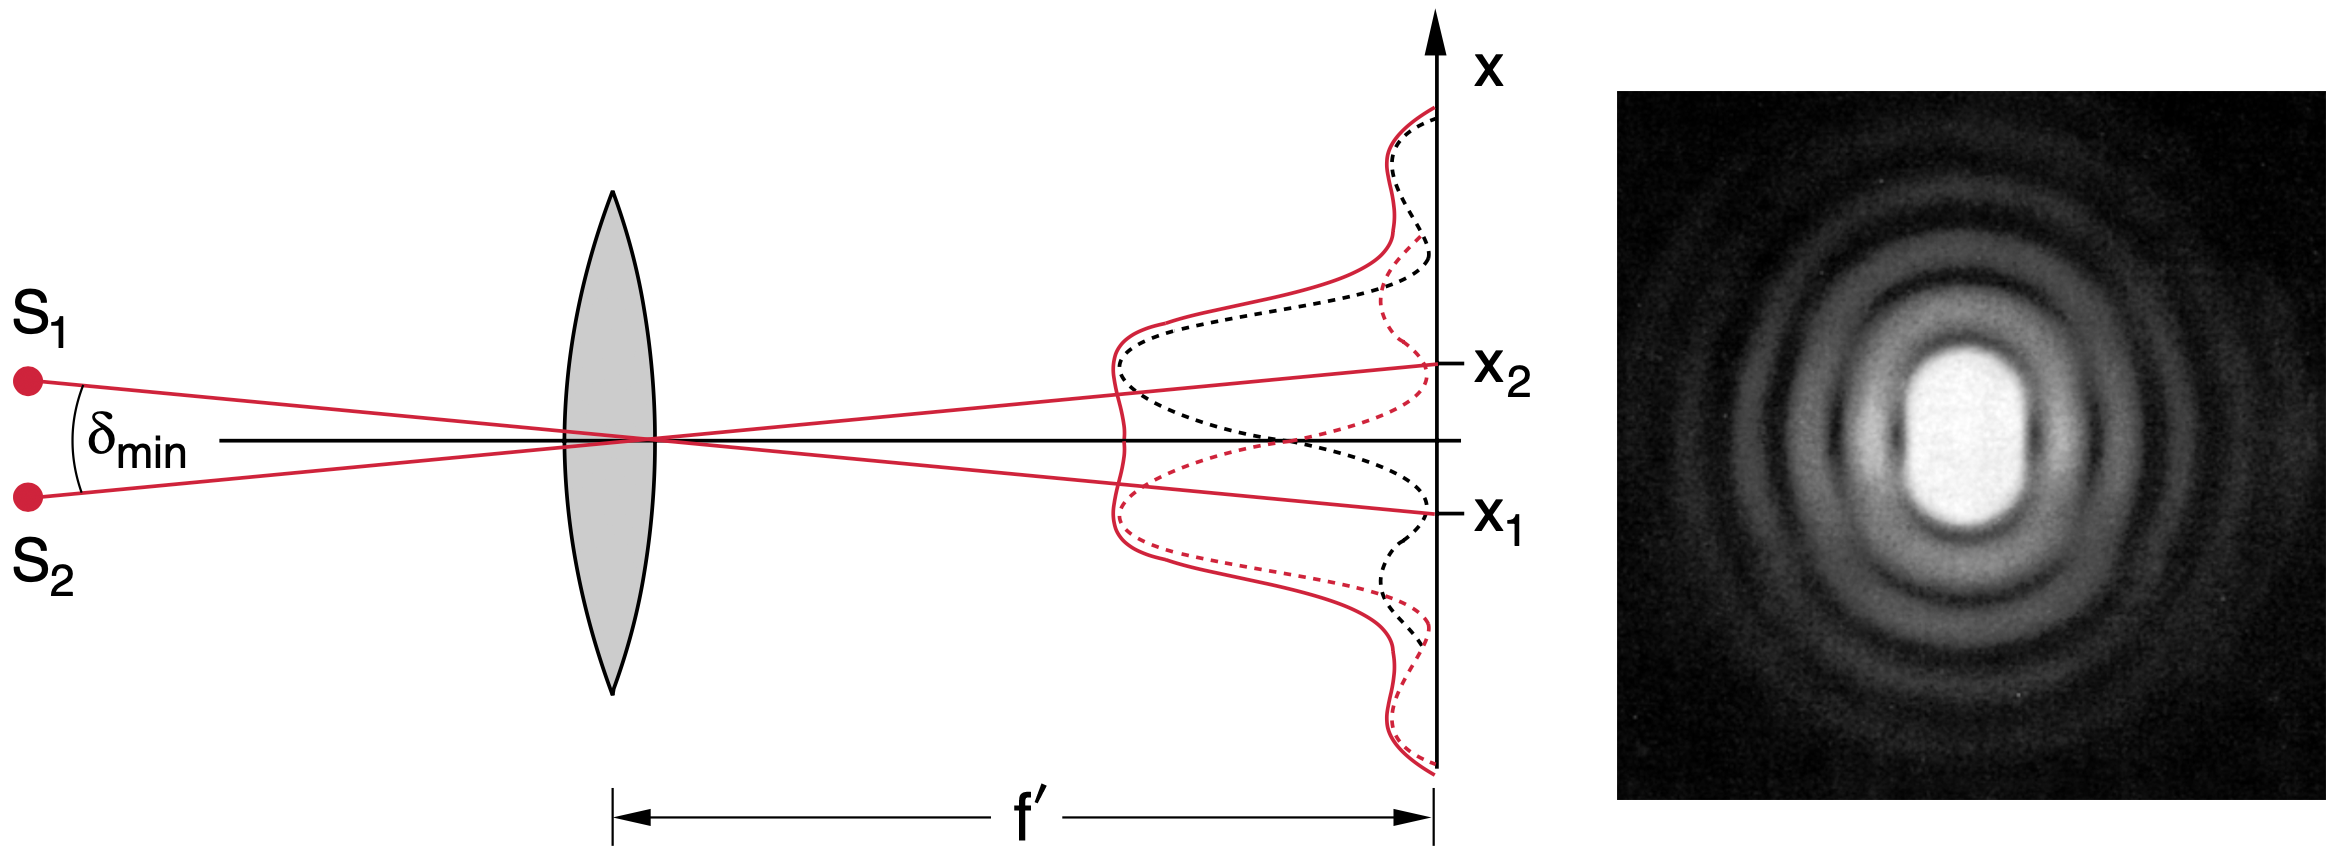
\includegraphics[width=\linewidth]{imgs/optics/airy-limit.png}
  \caption{The imaging subsystem is not capable of resolving two adjacent object points, leading to the interferences in the signal. Via \cite{Cagnet1962} and \cite{Demtroeder2018}.}
  \label{fig:airylimit}
  \Description{Two point sources are depicted in an imaging system and raytraced in a manner similar to the previous figure. The limits placed by diffraction cause the concentric patterns to overlap, rendering the two point sources spatially indistinguishable from each other.}
\end{figure}
%also, numerical aperture = n sin delta, with n = 1 bc air
The angular resolution of an optical system in an object plane is concomitant with a spatial resolution in an image representation, due to to the small-angle aproximations \cite{Pedrotti2007}. Defined via \textit{Rayleigh criterion}, the least resolvable distance between two points should correlate with the distance between the two peaks of the intensity distribution function (as seen in Figure \ref{fig:airylimit}):

\begin{displaymath}
  {\delta}'_{min} =  1.22 \lambda \frac{{f}'}{D} = 1.22 \lambda k \simeq {\rho}'_{\infty } 
\end{displaymath}

The latter is defined as the resolution limit ${\rho}'_{\infty}$ and can be approximated for the near field application, where the distance ${a}'$ between the aperture and the sensor plane is larger than the focal length ${f}'$:

\begin{displaymath}
{\rho}'_{near}  =  1.22 \lambda \frac{{f}'}{D} \frac{{a}'}{{f}'}= 1.22 \lambda k (1 - {\beta}' )
\end{displaymath}

The resolution limit presented earlier sets a limit for the peak lens performance, which varies with the fundamental physical quantities, like wavelength range and focal ratio.  
Further limitations are imposed through the geometric aberrations, caused by the physical imperfections in the optics itself.

The number of distinct resolvable points for a lens is defined by the \textit{space-bandwidth product} (SBP) \cite{Cossairt:11} and ties the lens performance to the sensor size.

\cite{GigaOptik} state two common approaches for enhancing the SBP. Those consist of either scaling the system up, or introducing further optical surfaces to the imaging system for better lens performance. The scaling can occur in either one of the subsystems, meaning an integration of a sensor with larger dimensions or scaling the lens.%, which are said to have SBP quadratic... aus scaling laws 
The second measure should lessen influence of geometric aberrations, leading to a diffraction-limited performance; however, the increased complexity of the optical system implies higher manufacturing costs and errors due to misalignment. Detailed description of scaling laws for the lenses is provided in \cite{Cossairt:11}, who account for both diffraction-induced limits and geometric aberrations.

As the CIS pixel sizes are routinely surpassing the 1.5$\mu$m extent, the optical system in a gigapixel application is doomed to have a lower resolving power than the sensor itself even if the lens performance is solely diffraction-limited; hence, the resolution in image space will be limited through optics. Resulting image representations contain spatial redundancies due to the light field being oversampled. 

While many proof-of-concept solutions exist that aim to enhance the resolution on a solely optical level (i.e., multiscale design and monocentric lenses), computational post-processing in gigapixel devices might turn out to be compulsory.
